\section{Introduction}
\label{sec:intro}

Sequence foundation models are increasingly applied to immune receptors
(T-cell receptors, antibodies, nanobodies) and to protein--protein interaction
(PPI) modelling. Evaluating such a model fairly requires a broad, reproducible
downstream panel that (i) distinguishes paper values, official artifacts, and
local reimplementations, and (ii) avoids rankings when splits, heads, metrics,
or seed protocols differ.

\begin{figure}[t]
\centering
\begin{subfigure}{\textwidth}
  \centering
  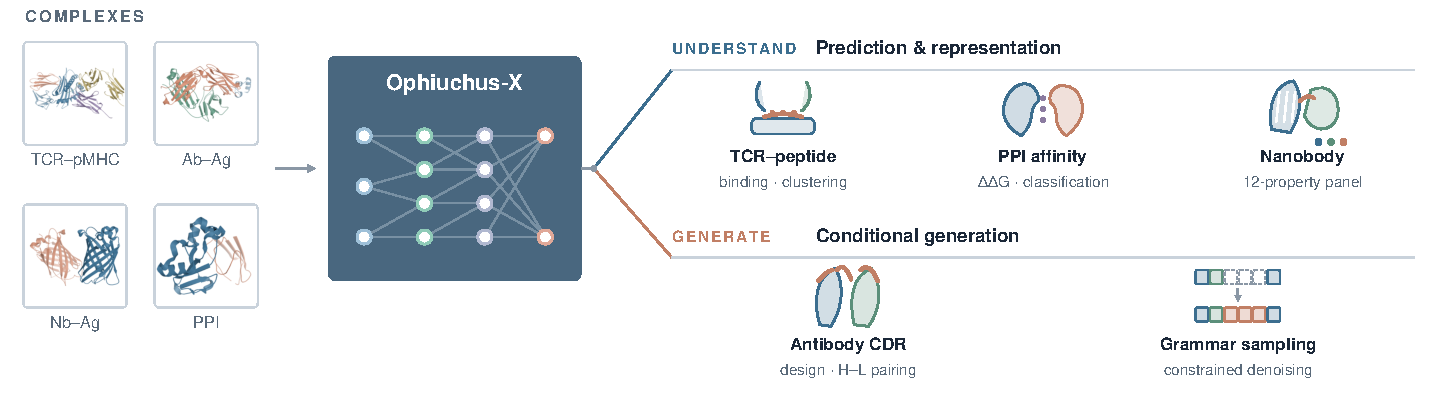
\includegraphics[width=\textwidth]{figures/fig1a_overview.pdf}
  \caption{A single frozen checkpoint serves both understanding (prediction /
  representation) and generation across TCR, antibody, PPI and nanobody tasks.}
  \label{fig:overview-a}
\end{subfigure}

\vspace{0.6em}
\begin{subfigure}{\textwidth}
  \centering
  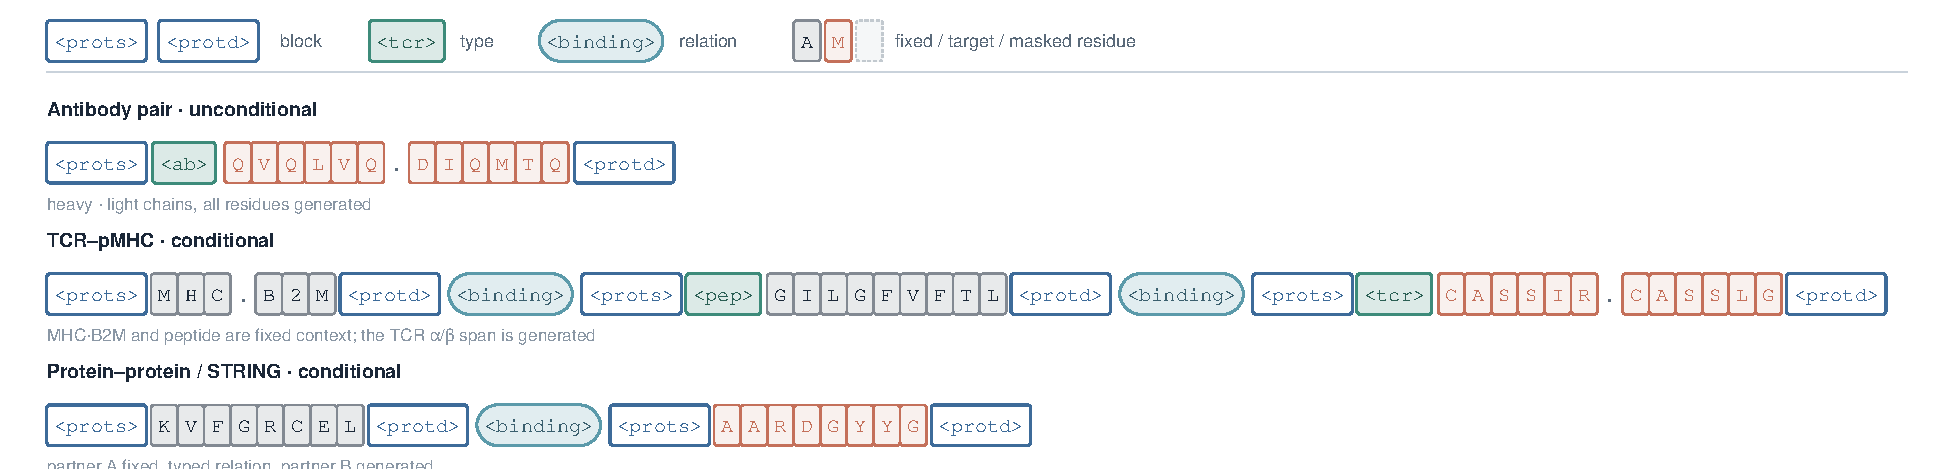
\includegraphics[width=\textwidth]{figures/fig1b_grammar.pdf}
  \caption{Designed grammar-v2 token format. Entity blocks
  (\texttt{<prots>}{\ldots}\texttt{<protd>}) carry an optional type tab and
  residue span; relation tokens join blocks. Grey residues are fixed context;
  orange residues are diffusion targets.}
  \label{fig:overview-b}
\end{subfigure}

\vspace{0.6em}
\begin{subfigure}{\textwidth}
  \centering
  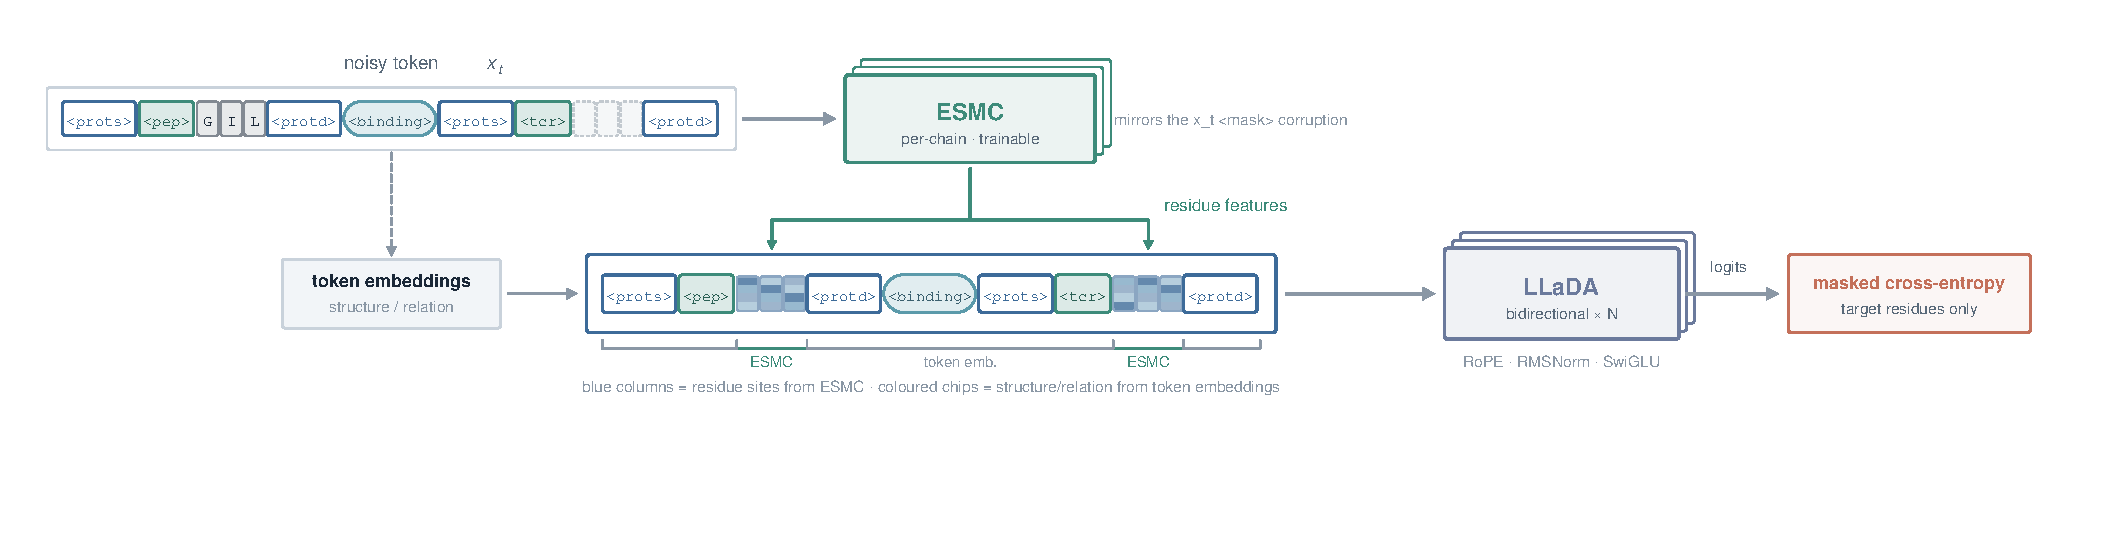
\includegraphics[width=\textwidth]{figures/fig1c_architecture.pdf}
  \caption{Training forward pass. Noisy tokens are read two ways: ESMC encodes
  each chain (corruption-mirrored) into residue features that replace embeddings
  at residue sites, while structure/relation tokens keep token embeddings; the
  fused stream enters a bidirectional LLaDA trained with masked cross-entropy on
  target residues.}
  \label{fig:overview-c}
\end{subfigure}

\vspace{0.6em}
\begin{subfigure}{\textwidth}
  \centering
  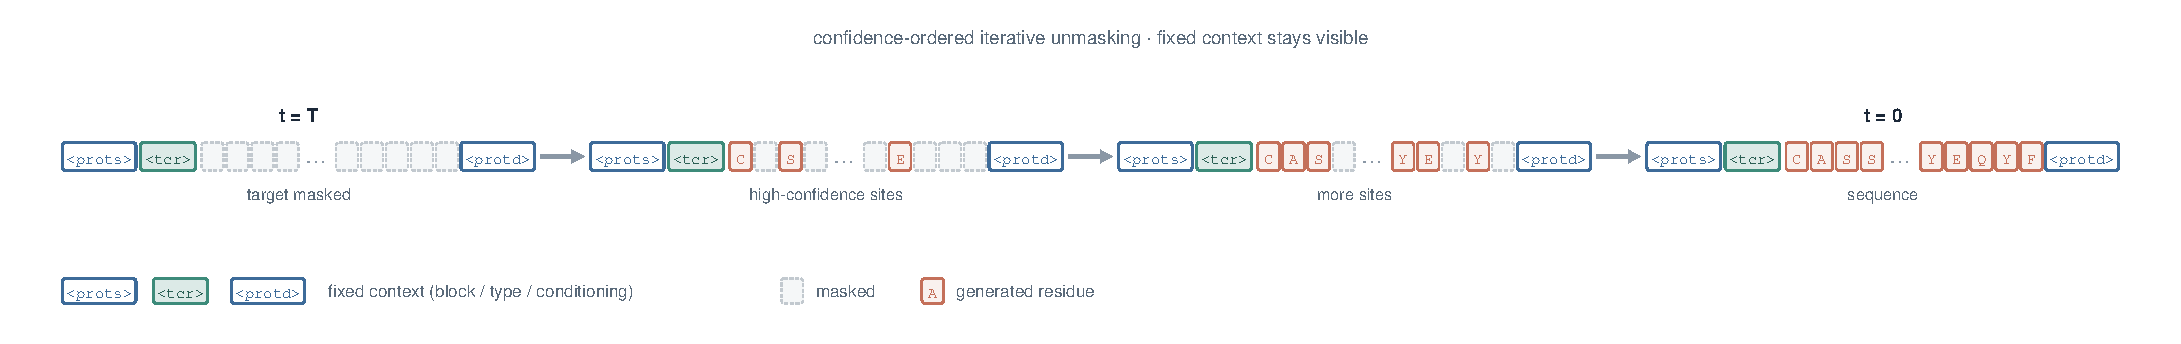
\includegraphics[width=\textwidth]{figures/fig1d_generation.pdf}
  \caption{Inference: confidence-ordered iterative unmasking. Fixed context
  stays visible while masked target sites are revealed from high- to
  low-confidence.}
  \label{fig:overview-d}
\end{subfigure}
\caption{Overview of \Ours{}, a grammar-conditioned ESMC$\rightarrow$LLaDA
diffusion language model.}
\label{fig:overview}
\end{figure}

This paper documents such a panel for \Ours{}, a grammar-conditioned
ESMC$\rightarrow$LLaDA diffusion language model (\Cref{fig:overview}). Our
contributions are:
\begin{itemize}
  \item \textbf{A unified, plug-in benchmark} (\Cref{sec:interface}) covering ten
  downstream tasks across TCR, PPI, antibody, and nanobody families, where any
  embedder is selected by a single string spec.
  \item \textbf{Source-labelled baselines and calibration.} Paper-reported
  values [P], official-artifact re-scores [A], and local evaluations [L] are
  kept separate. When a local protocol differs, [P] is the primary baseline.
  \item \textbf{A reusable evaluation harness} (\Cref{sec:experiments}): a single
  frozen checkpoint is plugged into every task via post-LLaDA feature extraction.
  We report the integrated 7-layer checkpoint honestly, including limitations on
  PPI classification, unseen-epitope generalisation, and conditional generation.
\end{itemize}
